% Introduction

\chapter{Introduction} % Main chapter title

\label{Introduction} % For referencing the chapter elsewhere, use \ref{Introduction}

%----------------------------------------------------------------------------------------

% Define some commands to keep the formatting separated from the content
\newcommand{\keyword}[1]{\textbf{#1}}
\newcommand{\tabhead}[1]{\textbf{#1}}
%\newcommand{\code}[1]{\texttt{#1}}
\newcommand{\code}[1]{\texttt{\hl{#1}}}
\newcommand{\file}[1]{\texttt{\bfseries#1}}
\newcommand{\option}[1]{\texttt{\itshape#1}}
\newcommand{\iBubble}{\textsc{iBubble}}
\newcommand{\rasp}{\textsc{Raspberry Pi}}
\newcommand{\vc}{\textsc{VideoCore iv 3D}}
\newcommand{\cpu}{\textsc{arm cpu}}
\newcommand{\bcm}{\textsc{bcm2837}}
\newcommand{\qpu}{\textsc{qpu}}
\newcommand{\flow}{\textsc{optical flow}}
\newcommand{\feat}{\textsc{feature}}
\newcommand{\api}{\textsc{api}}
\newcommand{\ram}{\textsc{shared ram}}
\newcommand{\mail}{\textsc{mailbox}}

%----------------------------------------------------------------------------------------

\section{\textsc{Notilo+} \& \textsc{iBubble}}

\footnote{\groupname{}: \url{https://ibubble.camera/}}\groupname{} is a young and innovative start-up based in Lyon. It was created in 2016 by Nicolas \textsc{Gambini} and Benjamin \textsc{Valtin} and early funded through crowd-funding during the 2016 year.

Currently about 20 people are working at \groupname{}. The company is divided into two parts: a business and commercial section and a technical section.

This technical section consists of an hardware-oriented team with mechanical and electronics engineers, an embedded sofware team of low-level developers and a vision team that I have joined. This team is composed of Filip the Computer Vision lead and my personnal supervisor, Loic a Computer Vision engineer, Nima a Robotics engineer and Camille a Computer Vision trainee.

The objective of \groupname{} is to develop and sell an \emph{autonomous} and \emph{wireless} underwater drone called \iBubble.

\begin{figure}[h]
\centering
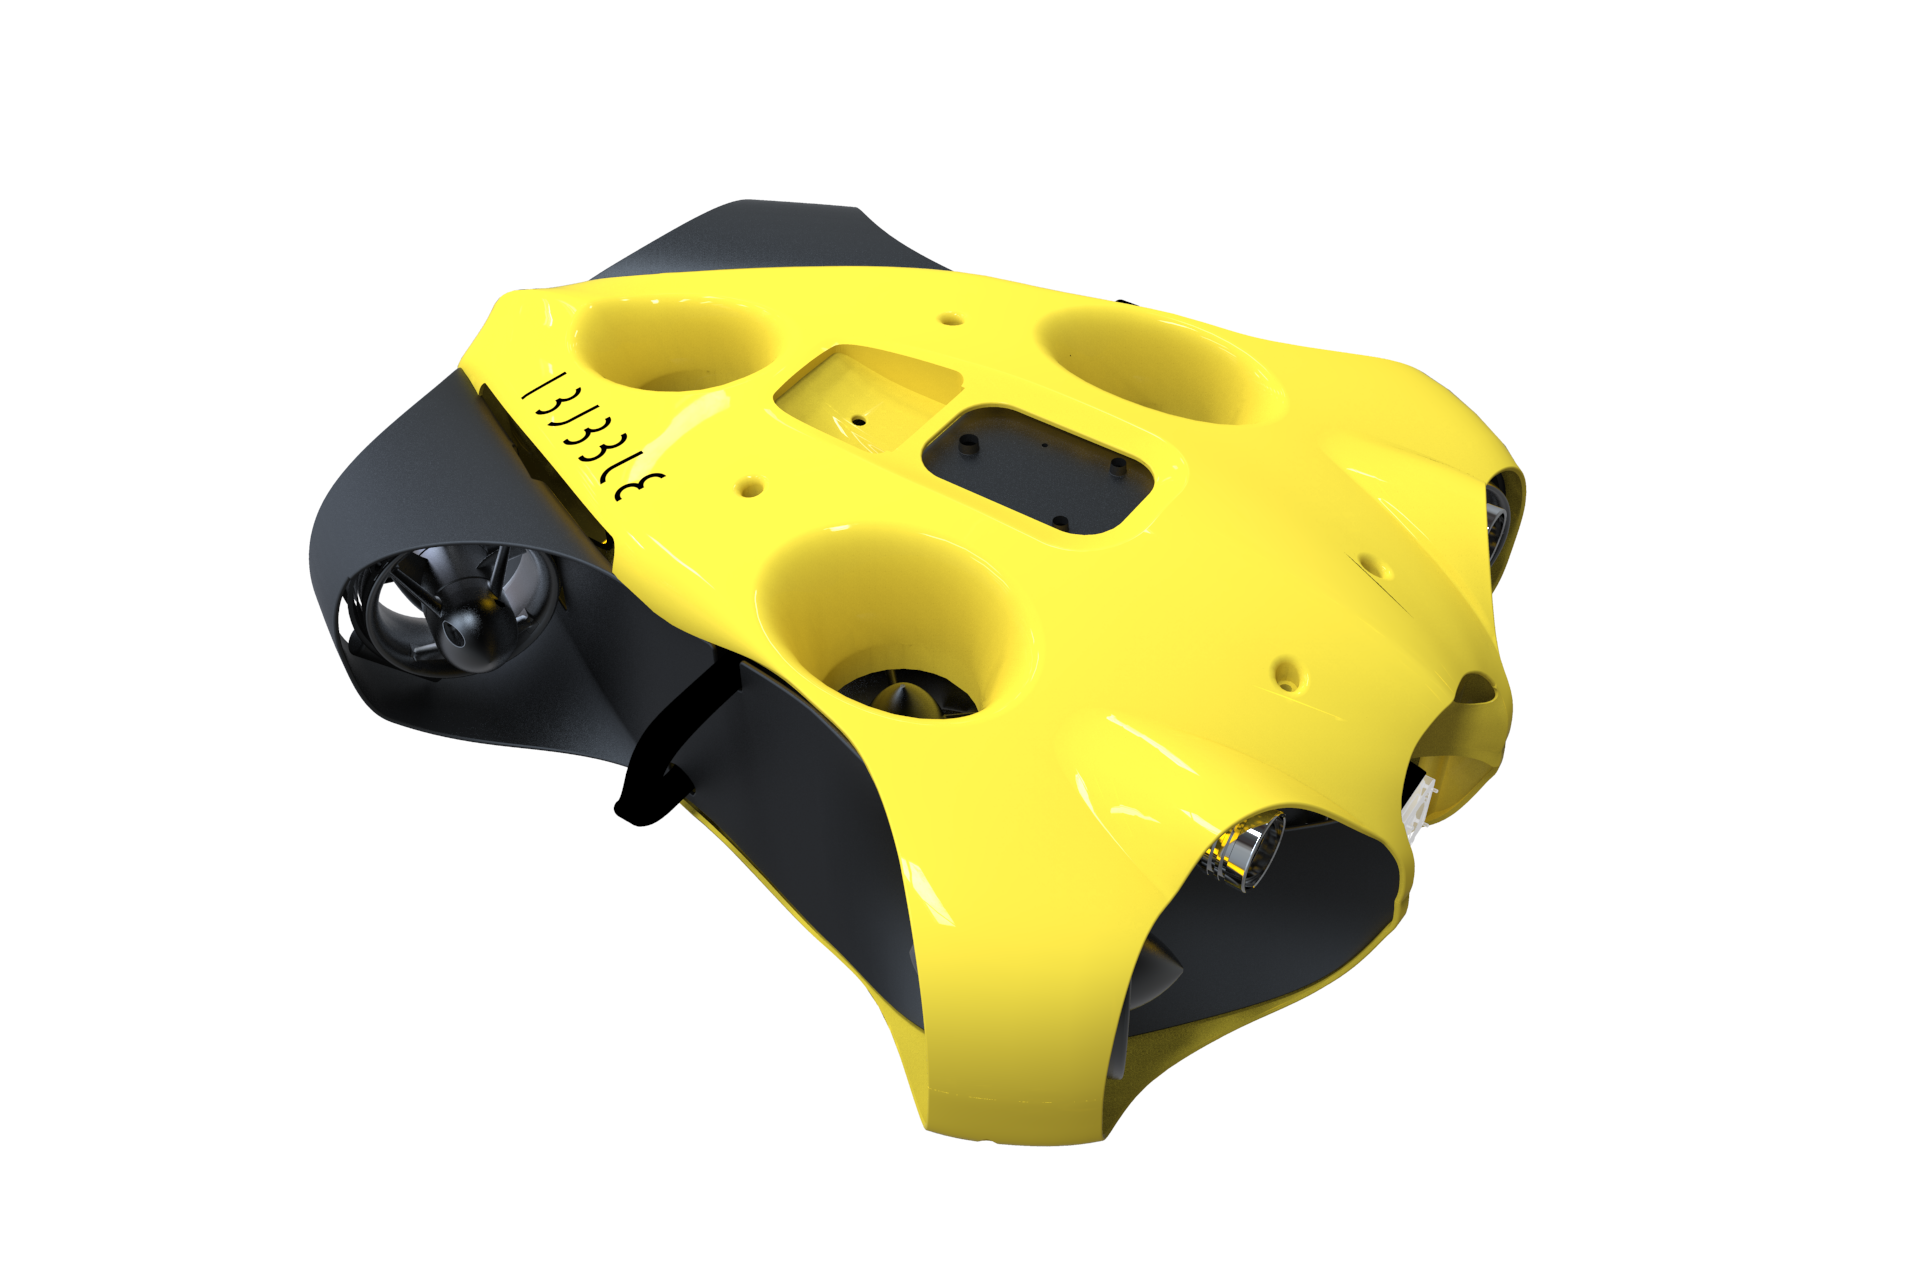
\includegraphics[width=0.4\textwidth]{iBubble3}
\caption{\iBubble{} drone}
\end{figure}


\iBubble{} is designed to replace cameraman divers. It can \emph{autonomously} follow a diver and capture footages from the diving session without any action from the user. The targeted \keyword{BtC} audience are for instance professional divers, diving centers, free-divers or resorts.

A live video feedback is also available on \iBubble. In this mode, a cable link between the drone and the user enables the video feedback on a smartphone and users can explore unknown spots before diving.\\


In addition to this \keyword{BtC} sector, \iBubble{} is suitable for a large range of \keyword{BtB} applications. Indeed, it can integrate multiple specific feat{}s for companies that have real needs in underwater inspection such as dam, harbor or simply ship's hull. Thanks to its \emph{autonomous} ability, it will be able to verify the good shape of a concrete wall for example and provides videos of its inspection.

%----------------------------------------------------------------------------------------

\section{Autonomous Tracking System}

As I said in the previous section, \iBubble's main feature is to follow \emph{autonomously} a diver to film the diving session. The diver can only choose one of the drone's available scenarii such as \emph{follow me}, \emph{circle me}, \emph{follow me side} etc. At any time the diver, or someone else is controlling the drone with a joystick. Because of the countless difficulties raised by underwater environments (no GPS, no Wi-Fi etc.), \emph{autonomously} follow a diver is a high technical challenge. To achieve this goal, \iBubble{} uses two technologies: \emph{acoustic} and \emph{vision} location.

The whole \iBubble's \emph{Autonomous Tracking System} -- acoustic and vision -- is implemented in a project called \keyword{NotiloTracker}.

\subsection{Acoustic System}

The diver is outfitted with a remote control that is an \emph{acoustic} emitter sending ultrasound pulses. \iBubble{} detects those pulses thanks to five \emph{acoustic} receivers and locates approximately the diver. This \emph{acoustic} positioning system is not very accurate because of the heavily perturbated underwater environment. As a consequence a \emph{vision} system is used to locate the diver in parallel.


\subsection{Vision System}

\label{Vision} % For referencing the chapter elsewhere, use \ref{Vision}

\iBubble{} has two cameras at his disposal: one to record the diving session (generally a \emph{GoPro} camera) and another one to capture frames used in the computer vision part. This camera is generally a cheaper camera with a low resolution. When \iBubble{} is opposite the diver it can detect the position more precisely thanks to several algorithms running on the embedded board.

The vision system is globally composed of two parts: a \emph{machine learning detector} to lock the position of the diver and a \emph{tracker} to follow him between two frames of the video. The bulk of complexity is to compute the \flow{} for the \emph{tracking} algorithm and in Forward Propagation of a Convolutional Neural Network for the \emph{detector} algorithm.

%----------------------------------------------------------------------------------------

\section{Internship}

\subsection{Problematics}

The vision algorithms mentionned in~\ref{Vision} are well-known and can be parallelize very efficiently on \keyword{GPU}s to improve compute speed. Therefore there are a lot of implementations on \keyword{GPU}s of these algorithms especially with the growth of \emph{Nvidia's CUDA GPGPU cores} on embedded chip (for instance the Jetson TX2 board).

However, \groupname{} chose \rasp\footnote{Raspberry Pi: https://www.raspberrypi.org/} as the central embedded computer for \iBubble. Indeed, this board is far less expensive than \emph{CUDA} systems, reasonably powerful and very well-documented with a huge community of developers.\par

The \keyword{SoC} used in the \rasp{} is a \keyword{\textsc{Broadcom}} \bcm{}\footnote{BCM2837: \url{https://www.raspberrypi.org/app/uploads/2012/02/BCM2835-ARM-Peripherals.pdf}} fitted with:
\begin{itemize}
\item \keyword{CPU} -- \keyword{ARM Cortex A53} (ARMv8) cluster
\item \keyword{GPU} -- \vc{}
\end{itemize}

Furthermore, the current vision system (\emph{detector \& tracker}~\ref{Vision}) uses state-of-the-art algorithm \keyword{CMT}\footnote{CMT algorithm: \url{https://www.gnebehay.com/cmt/}}, developed with \keyword{OpenCV}\footnote{OpenCV: https://opencv.org/} the main library used in Computer Vision.

The main issue is that the \bcm{} is not designed with a \emph{CUDA} architecture and there is no reliable implementation of the algorithms on the \rasp. As a consequence, the \vc{} can't be used and the whole \emph{tracking system} is running only on the \rasp's \keyword{CPU}, resulting in slow computing time and poor performances. Since all the vision system will be integrated on the \rasp, the difficulty is to achieve correct quality with a real-time processing on a such device.

To meet these objectives, \groupname{} have decided to developp its own implementation of those algorithms using an homemade \keyword{API} for the \vc. This is the subject of my internship.


\subsection{Subject}

From low-level programming to image processing and numerical analysis, this subject covers a wide range of fields. Therefore, the internship work has been split into two internships:

\begin{itemize}
\item \keyword{API} for the \keyword{GPU}: with my background on embedded systems, I was focused on the \vc{} programming
\item Algorithms Implementation: another intern, Camille \textsc{Farineau}, was focused on the \keyword{tracking \& detctor} algorithms implementation
\end{itemize}


\subsubsection{Algorithms Implementation}

Camille's job was to work on:

\begin{itemize}
	\item \emph{Machine Learning} algorithm for the \emph{detector}
	\item \flow{} computation -- part of \keyword{CMT} algorithm -- for the \emph{tracker}
\end{itemize}

Indeed, before implementing these algorithms on the \vc, it was crucial that \groupname{} has its own implementation of them. Currently all the vision system is coded in \keyword{C++} and uses libraries such as \emph{OpenCV}. Camille had to work on these algorithms with the technologies, libraries, frameworks that fit the best the problem, namely processing parts of these algorithms on the \vc{} in order to release some \keyword{CPU} ressources.

In a first time he has to study and understand the popular implementations of the \flow{} algorithms, create a state-of-the-art document of these algorithms. Then he suggests an optimized implementation for the chosen method. This implementation must be highly parallelizable in order to use the \vc. At this stage, wa have to communicate together so that I understand how the \vc{} can be helpful for the implementation of the \flow{} algorithm.

Next this algorithm needs to be test in simulation and real conditions on the \rasp. This step is fundamental to estimate the gain and loss in quality and computing time compared to the current solution. Finally the last part is to implement it on the drone system and test the whole vision system with the new \flow{} algorithm.


\subsubsection{API for the \textsc{VideoCore IV 3D GPU}}

Personnaly I had to study and understand the \vc{}. The goal was to create an homemade \keyword{API} accessible from a high-level language such as \keyword{C++}. This \keyword{API} was to provide basic functions to run computations of the \flow{} algorithm on the \vc{} in order to achieve a real time performance and relieve the \keyword{CPU}.

Due to the growing popularity of the \rasp{}, \keyword{\textsc{Broadcom}} released an official \vc{} architecture reference guide\footnote{\vc{} Documentation: \url{https://docs.broadcom.com/docs/12358545}}, but without any official \keyword{API}.

As a conseqence, the main questions for me was to study the architecture and understand how to use the \vc{}, then understand the \flow{} algorithm and implement an optimized and parallelized version running on the \vc{}.

Camille and I worked in parallel but we had to coordinate ourselves in order to develop the dedicated functions. Camille had to specify the needs for the \flow{} algorithm (what kind of computations such as a convolution, gradient or interpolation functions etc.) and I have to adapt the \keyword{API} to integrate these functions on a program running of the \vc.

%----------------------------------------------------------------------------------------
